\section{Solar Coordinates - Will}
\label{sec:coords}
% edited by Steven C. 25-Apr-2019
% edited by Will B. 19-Apr-2019

The \package{sunpy.coordinates} subpackage provides definitions of and transformations between several reference frames commonly used in solar physics.
These reference frames and their associated transformations are implemented using the \package{astropy.coordinates} subpackage and extend \astropy's coordinate frame transformation graph to include solar coordinates.
\autoref{fig:transform_graph} shows the transformation graph between the various coordinate frames provided by \sunpy and their connection to astronomical coordinate frames.
Four solar physics coordinate frames are currently implemented: \hpc, \hcc, \hgs, and \hgc.
Each of these frames and the associated transformations are defined in \citet{2006A&A...449..791T}.
Both the \hpc and \hcc frames are observer-dependent and require the location of an observer to be specified when constructing the frame.
In the \hpc frame, the observer is at the origin of the coordinate system while in the \hcc frame the $z$-axis is defined to be parallel to the Sun-observer line.
% elaborate a bit more here as well; why are these frames useful? (split into two paragraphs)

% Description of the HCRS <-> HGS transform? - Stuart Mumford, Albert Shih?

\begin{figure}
    % Why are the arrows between the solar frames brown and green? all black?
    \centering
    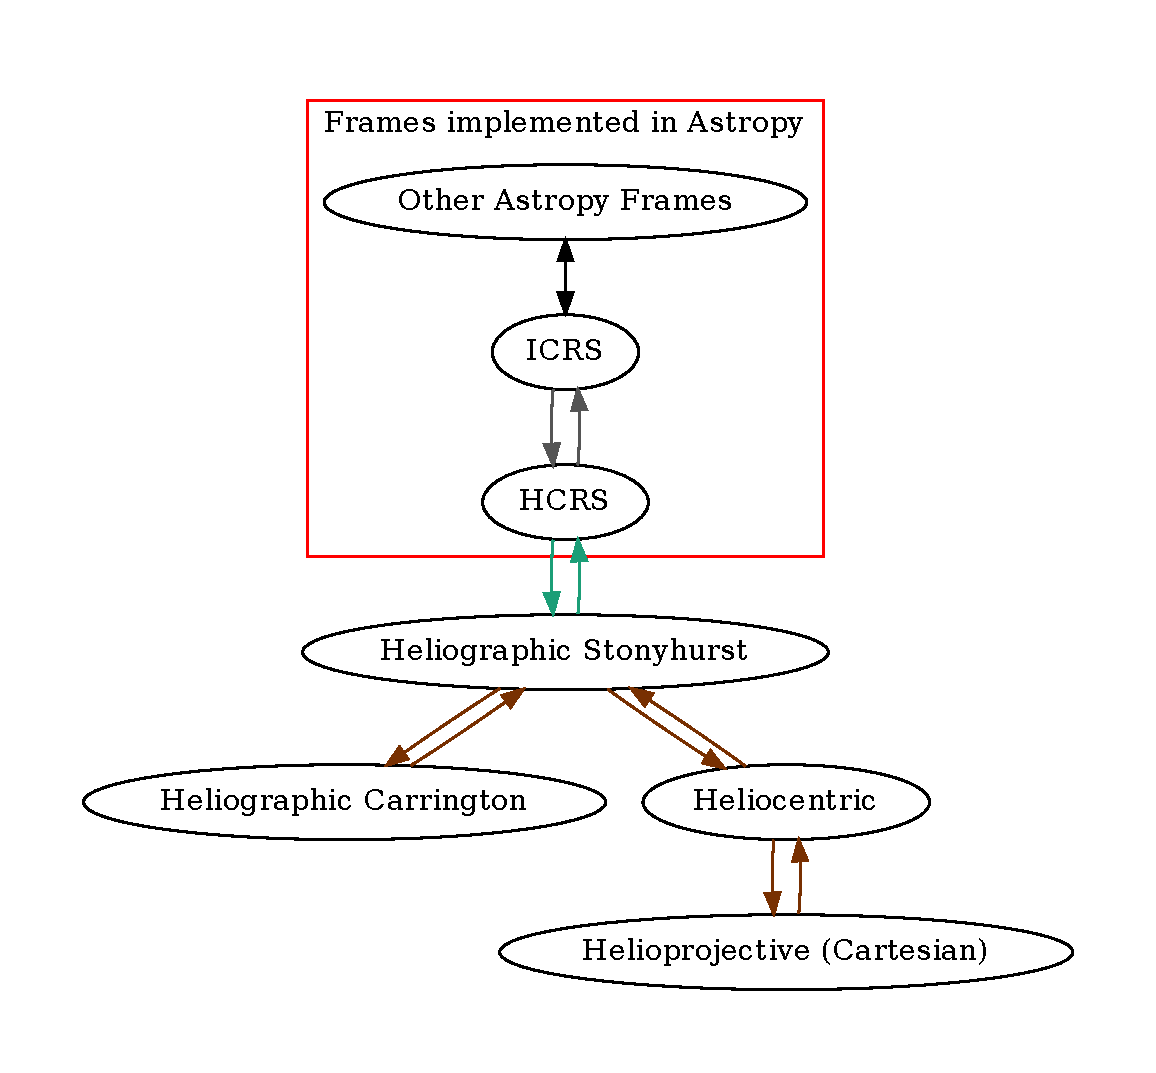
\includegraphics[width=0.75\textwidth]{figures/sunpy_frames.pdf}
    \caption{Graph of possible transformations between reference frames as implemented in \package{sunpy.coordinates}.
    The arrows indicate transformations between the different frames.
    Note that coordinates can be transformed to more general astronomical coordinate frames via the \hgs frame.}
    \label{fig:transform_graph}
\end{figure}

Coordinates and their associated frames are specified using an \astropy \code{SkyCoord} object \citep[see Section 3.3 of][]{astropy2018}.
Observer location is encoded in the same way.
For example, in the \hpc and \hcc frames, the \code{.observer\_coordinate} attribute is a \code{SkyCoord} defined in the \hgs frame.
The default observer location is set to the position of the Earth as long as the time of the observation is specified.
If the time is not set the coordinate cannot be transformed to another frame unless an explicit observer is specified, as the time is required to calculate the location of the Earth.
% elaborate on this a bit

The \package{sunpy.coordinates} subpackage is most useful when combined with the \sunpycode{Map} object (see \autoref{sec:map}).
Coordinates are automatically populated when opening a FITS image using the appropriate header metadata.
This combination enables a number of number of tasks which were once cumbersome.
A few examples are shown in \autoref{fig:coordinates_examples}.
% brief description of figures

%Just as an \code{astropy.units.Quantity} object is used to attach units to a numerical value (see \autoref{sec:units}), an \code{astropy.coordinates.SkyCoord} object includes the spatial coordinate as well as the system in which that coordinate is defined. In addition to the numerical values of the coordinate, a \code{SkyCoord} includes a reference frame or system and a representation. A reference frame describes the manner in which a point is oriented in space while a representation is a way to describe a point in a particular reference frame (e.g. Cartesian, spherical).

\begin{figure}
    \gridline{\fig{figures/fieldlines_aia.pdf}{0.3\textwidth}{(a)}
              \fig{figures/fig_venus_transit_1600_20120606_040729.pdf}{0.3\textwidth}{(b)}
              \fig{figures/fig_coronagraph_starfield.pdf}{0.3\textwidth}{(c)}
              }
    \caption{Several example use cases of the coordinates machinery in \sunpy.
    (a) Field lines traced from a field extrapolation of active region NOAA XXXX computed using \package{pfsspy} overlaid on an 171 \AA image from AIA.
    (b) The Venus transit as viewed by SDO/AIA in 1600 \AA. The predicted position of Venus is overplotted in helioprojective coordinates of the AIA image.
    (c) A coronagraph image of the solar corona as observed by STEREO-A COR-2. The predicted positions of the stars from the Gaia DR2 catalog and mars are overplotted.}
    \label{fig:coordinates_examples}
\end{figure}

\subsection{Solar differential coordination - Jack}
One paragraph long.
Not clear if it needs to be in this location.
Should it be in a map utility section?

Don't forget to refer to the figure!
An important application of....
Figure \ref{fig:diff_rot}


\begin{figure}
    \center
    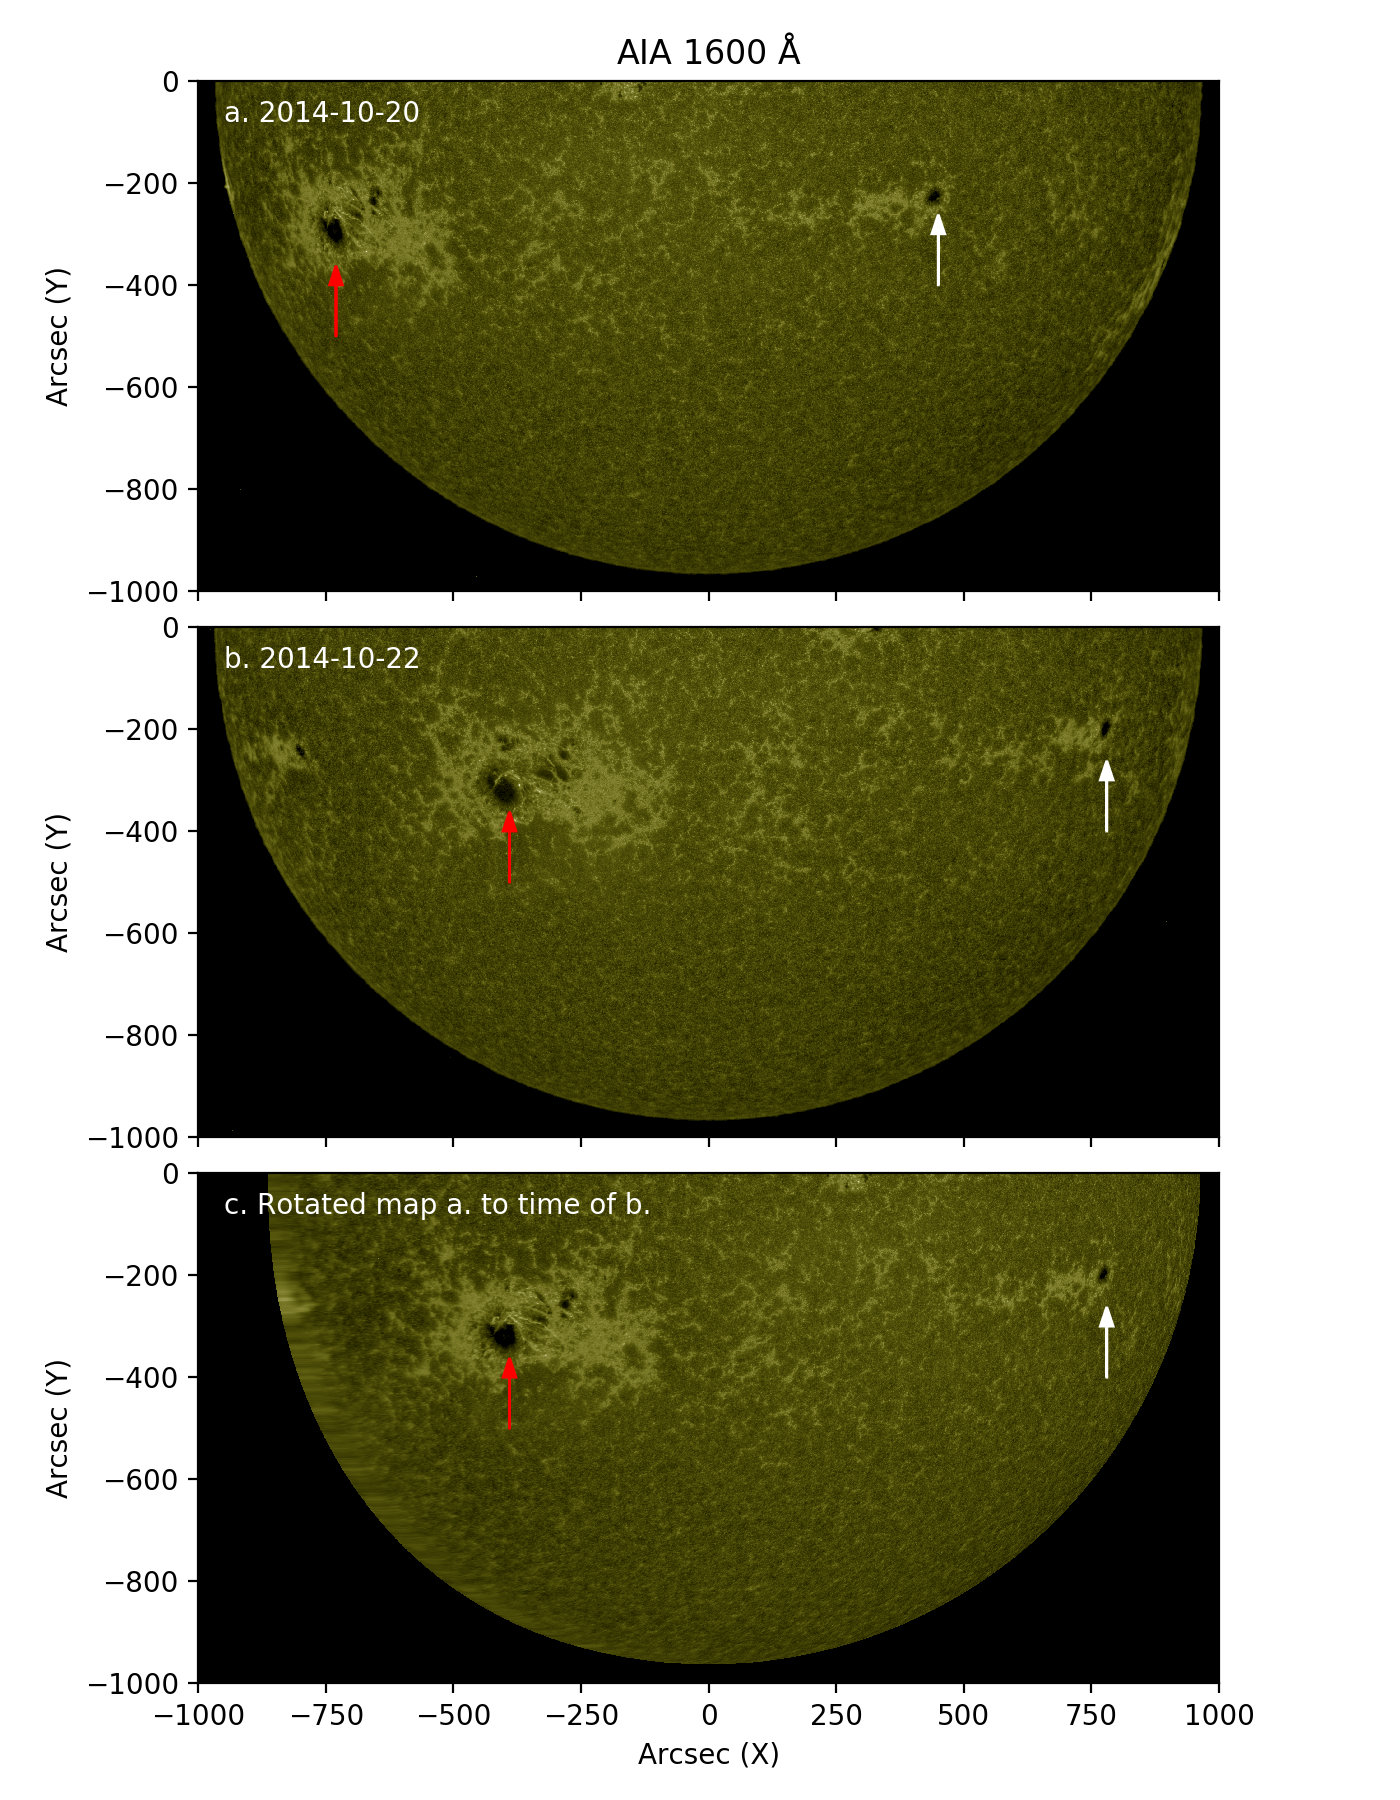
\includegraphics[width = 0.8\textwidth]{figures/diff_rot_aia1600.png}
    \caption{Example of the functionality of \sunpy to apply solar differential rotation to a Map.
    Panels (a) and (b) show the Sun as observed in AIA 1600~\AA\ on two different days, 2014-02-20 and 2014-02-22.
    A large sunspot group is highlighted by the red arrow, and a smaller sunspot by the white arrow.
    Panel (c) shows the map of (a) that has been rotated differentially using \sunpy to the time of map (b).}
    \label{fig:diff_rot}
\end{figure}
